\section{Introduction}

The design of stochastic models of distributed system has a long history as a challenging area of interest. Models of distributed systems have to deal with a number of factors. These factors include the various types of failure the system could experience, a lack of tightly synchronized execution, and a large complex state space when there are a high number of agents.  However, the concept of distributed systems plays a central role in many of the future visions for how critical infrastructure will operate in the near future. Computational systems already play a critical role in most critical infrastructures, and as demands for security features such as availability increase, distributed systems become an increasingly favorable choice for the computational needs for these systems.

The FREEDM smart-grid project follows this vision. The FREEDM center, an NSF funded ERC envisions a future power-grid where widely distributed renewable power generation and storage is closely coupled with a distributed system that facilitates the dispatch of power across those areas. Other systems like VANETs and Air Traffic control also propose similar control systems where many computers must co-operate to ensure both smooth operation, and the safety of the people using those systems. Because of this, ensuring the behavior of the computer systems that control these infrastructures behaves correctly during failure is critical, especially when those computer systems rely on their interaction with other computers to operate.

In a smart-grid system, misbehavior during fault conditions could lead to critical failures such as a blackout or voltage collapse. In a VANET or air traffic control system, vehicles could collide, injuring passengers or destroying property. Additionally, since these systems are a part of critical infrastructure, protecting them from malicious entities is an important consideration.

A stochastic model for a cyber-physical system is valuable while the system is being developed, but also valuable when the system is deployed in the field. [CITE] shows an application of a stochastic model in a smart-grid system being used to harden the system to protect it from message delay caused by congestion. This hardening changed the behavior of the cyber component of the CPS to allow its operation to continue (albeit with slightly different properties), while still protecting the physical system from errors that would have occured, had the system continued without hardening for those errors.

Therefore, it is valuable for the cyber-physical system to make its own stochastic models online and make decisions about how the agent should behave. However, typically, a well designed model requires an omnipotent view of the system. In distributed systems, this is particularly difficult as an instantaneous snapshot of the system is not possible without perfectly synchronous execution. Furthermore, while many algorithms for casual snapshots exist, a causal snapshot may not represent a state that the system was ever in. Additionally, taking these snapshots takes time and a model generated from that snapshot may not be viable by the time all the requisite information has been collected.

It is desirable then, to design distributed algorithms some agent can infer the state of other agents and generate a stochastic model of the future from those inferences. Then, using that model the agent can make decisions about how best to react to the current physical or cyber conditions that best benefits the CPS as a whole. However, the dispersal of information in a distributed system requires messages to be passed between agents, which can be disrupted by failure. The agent creating the stochastic model must be able to infer the state of the other agents it is attempting to model in order to create the model.

In this work, we present a framework for reasoning about inferable state in the context of a distributed system. To do this we exploit existing work in the field of information flow security. Information flow security has been used to reason about how attacks like STUXNET can manipulate operators beliefs while disrupting the system. In particular, these approaches reason about how the operator in a STUXNET attack has no avenue to verify the reports from a compromised computing device. Using existing modal logic frameworks and using information flow security models, one can formally reason about where information that is not normally known to a domain can be inferred.

We will show in this work that in a system with the correct information flows, an agent in a distributed system can infer the state of other agents in the system. With this information, that agent can then construct a reasonable model of the system to determine if the current behavior could lead to an undesirable situation with either the cyber or physical network. We formalize how this flows are created using information flow security models.

\section{Background}

\subsection{Information Flow Security}

\subsubsection{Modal Logic}

Kripke frames play a critical role in the development of this work. The essential concept of this work is that each global state of the distributed system at any given instant can be captured as a countably infinite set of propositional variables. A Kripke frame is a pair <W,R> such that W is a set of of possible versions of the global state over time, where each element in $W$ is known as a world. Each element of $R$ describes a binary relationship for how the described system can move from world to world as events occur in the described system.

In the case of a distributed system, a world could be described as one the possible combinations of values of all boolean state variables $S=\{s_0, s_1, ... s_n\}$ in that system. As execution occurs, messages, time, or events cause these variables to change. Each change in boolean variables corresponds to a relationship in R. Therefore, a world $w$ is one possible valuation of all the variables in s and a transition from $w$ to another $w'$ (with its own valuation) can be noted as $wRw'$. Without loss of generality, each relationship in $R$ must result in the change of at least one variable in $S$. Additionally, the set of world is complete: every possible combination is represented in the set of worlds. No relationship can lead to a world that does not exist.

Additionally, we can define a set of valuation functions, $\{V\}$. Each function $V^i_{s_x}$ in $V$ describes the value observed by an agent $i$ of a boolean state variable $s_x$.  If a valuation function for a particular state variable is not defined for an agent, that agent cannot determine the value of that state variable, and cannot determine the value of any logical statement based on that variable. In the case of a distributed system, this concept is analogous to the isolation of memory for each agent. For example, an agent $i$, cannot simply determine the value of a variable for agent $j$.

The combination of a Kripke Frame $< W,R >$ and a set of valuation functions ${V}$ is a Kripke Model $M = \{W, R, V\}$ sometimes known as a modal model. The complete model describes all the possibilities that the modeled system can go through.

Let $\varphi \in \Phi_0$ be an atomic proposition in a set of countably many propositions. The set of well-formed formulas (wffs) as defined by the formulation rules in \ref{tab:axiomatic} is the least set containing $\Phi_0$. Additionally, we use the modal operator $\Box$ as an abbreviation for $\neg \Diamond \neg \varphi$. The complete axiomatic system is outlined in \ref{tab:wffs}. For the uninitiated, the modal box operator ($\Box$), ``it is neccesary that'' states (in the case of $\Box \varphi$) that in every world $w$, $\varphi$ is true. As its dual, the diamond operator ($\Diamond$) states, that it is not the case that in every world, $\varphi$ is true.

\begin{table}[]
\small
\centering
\caption{Logical Statement Formulation Rules}
\begin{tabular}{r l}
1. & if $\varphi$ is a wff, so are $\neg \varphi$, $\Box \varphi$, and $\Diamond \varphi$. \\
2. & if $\varphi$ is a wff, so are $B_i \varphi$ and $\neg B_i \varphi$ \\
3. & if $\varphi$ is a wff, so are $T_{i,j} \varphi$ and $\neg T_{i,j} \varphi$ \\
4. & if $\varphi$ is a wff, so are $I_{i,j} \varphi$ and $\neg I_{i,j} \varphi$ \\
5. & if $\varphi$ and $\psi$ are both wff, so are $\varphi \wedge \psi$ \\
6. & if $\varphi$ and $\psi$ are both wff, so are $\varphi \vee \psi$ \\
\end{tabular}
\label{tab:wffs}
\end{table}

\begin{table}[!t]
\small
\centering
\caption{The Axiomatic System}
Definition of logical and modal operators (abbreviations) \\
\begin{tabular}{r l}
D1. & $\varphi \wedge \psi \equiv \neg ( \neg \varphi \vee \neg \psi)$\\
D2. & $\varphi \oplus \psi \equiv (\varphi \vee \psi) \wedge \neg(\varphi \wedge \psi)$ (exclusive or)\\
D3. & $\varphi \rightarrow \psi \equiv \neg \varphi \vee \psi $\\
D4. & $\varphi \leftrightarrow \psi \equiv (\varphi \rightarrow \psi) \wedge (\psi \rightarrow \varphi)$\\
D5. & $\Diamond \psi \equiv \exists w \in W : w \vdash \varphi $\\
D6. & $\Box \varphi \equiv \neg \Diamond \neg \varphi $\\
D7. & $B_i \varphi$ agent $i$ believes the truth of $\varphi$\\
D8. & $I_{i,j} \varphi$ agent $j$ informs $i$ that $\varphi \equiv \top$\\
D9. & $T_{i,j} \varphi$ agent $i$ trusts the report from $j$ about $\varphi$ \\
\end{tabular} \\~\\
Axioms \\
\begin{tabular}{r l}
P. & All the tautologies from the propositional calculus.\\
K. & $\Box (\varphi \rightarrow \psi) \rightarrow (\Box \varphi \rightarrow \Box \psi)$\\
M. & $\Box \varphi \rightarrow \varphi$\\
A1. & $\neg \Box \varphi \rightarrow \Box \neg \Box \varphi $\\
A2. & $\Diamond (\varphi \vee \psi) \rightarrow \Diamond \varphi \vee \Diamond \psi $\\
A3. & $\Box \varphi \wedge \Box \psi \rightarrow \Box (\varphi \wedge \psi)$ \\
B1. & $(B_i \varphi \wedge B_i (\varphi \rightarrow \psi )) \rightarrow B_i \psi$ \\
B2. & $\neg B_i \bot$\\
B3. & $B_i \varphi \rightarrow B_i B_i \varphi$ \\
B4. & $\neg B_i \varphi \rightarrow B_i \neg B_i \varphi$\\
I1. & $(I_{i,j} \varphi \wedge I_{i,j} (\varphi \rightarrow \psi )) \rightarrow I_{i,j} \psi$\\
I2. & $\neg I_{i,j} \bot$ \\
C1. & ($B_i I_{i,j} \varphi \wedge T_{i,j} \varphi) \rightarrow B_i \varphi$ \\
C2. & $T_{i,j} \varphi \equiv B_i T_{i,j} \varphi$ \\
\end{tabular} \\~\\
Rules of Inferrence \\
\begin{tabular}{r l}
R1. & From $\vdash \varphi$ and $\vdash \varphi \rightarrow \psi$ infer $\psi$ (Modus Ponens) \\
R2. & $\neg (\varphi \wedge \psi) \equiv (\neg \varphi \vee \neg \psi)$ (DeMorgan's)\\
R3. & From $\vdash \varphi$ infer $\vdash \Box \varphi$ (Generalization)\\
R4. & From $\vdash \varphi \equiv \psi$ infer $\vdash \Box \varphi \equiv \Box \psi$\\
R5. & From $\vdash \varphi \equiv \psi$ infer $\vdash T_{i,j} \varphi \equiv T_{i,j} \psi$\\
\end{tabular} \\
\label{tab:axiomatic}
\end{table}

\subsubsection{Non-Deducible (MSDND) Security}

In the domain of security concepts there are a wide variety of goals worth protecting in every system. These include the core security concepts of integrity, accessibility and privacy. Most traditional security approaches rely heavily on cryptography to provide privacy. However accidental information leakage can still occur, which compromises the privacy of the system. For cyber-physical systems, the leakage is difficult to control. Unlike their cyber counterparts, the actions taken by the physical components cannot be hidden from a casual observer. For example, a plane changing altitude or a car turning or changing speed cannot be hidden from an observer. Other, more complicated systems, like the power grid, have actions that are more difficult to observe, but a well motivated attacker can potentially collect critical information about the behavior of the cyber components with observations of the physical network.

Information Flow security models are invaluable for assessing what information, if any, is leaked by either the cyber of physical components of the CPS. There are a number of information flow security models, all based off similar concepts. Typically, these models partition the system into two domains: the high security domain and the low security domain. However, the MSDND security model allows the system to partitioned into any number of domains. The MSDND model has been used to describe how the STUXNET attack was able to hide its malicious behavior from the operators. The MSDND security model is expressed using modal logic to determine what information in a domain is deducible to an observer in another domain. MSDND security exploits the possible worlds of modal logic to determine if there are worlds where the value of a logical atom is deducible by someone outside the domain.

This information flow security model can be used to determine what an agent in a distributed system can determine about another agent. The exact specification of timing the distributed system becomes unnecessary as the modal model can express any combination of logical atoms in one of its worlds. 

The MSDND security model can be expressed as follows. Consider a pair of state variables $s_x$ and $s_y$ which may or may not be in the same security domain. The value of $s_x$ and $s_y$ have a logical xor relationship: if $s_x$ is true, $s_y$ must be false. Given an agent $i$ that does not have a valuation function for either of those two variables, the system is MSDND secure for that agent and pair of variables. Written formally:

\begin{align}
MSDND = \exists w \in W : w \vdash \Box [ (s_x \vee s_y) \wedge \neg(s_x \wedge s_y) ] 
\nonumber \\ \wedge [ w \vDash ( \not \exists V_x^i (w) \wedge \not \exists V_y^i (w) ) ]
\end{align}

Of particular interest is the special case where $s_x$ and $s_y$ are relation on the same wff: $(s_x = \varphi$ and $s_y = \neg \varphi)$:

\begin{align}
MSDND = \exists w \in W : w \vdash \Box [ \varphi \oplus \neg \varphi ] 
\nonumber \\ \wedge [ w \vDash ( \not \exists V_\varphi^i(w)) ]
\end{align}

In a system where the above logical relationship holds, the agent $i$ cannot determine the value of $s_x$ or $s_y$. However, if the relationship does not hold, there is some world where the agent can determine the value of $s_x$ and $s_y$.

\subsubsection{Belief Logic}

BIT was developed by such and such to formalize a modal logic about belief and information transfer. BIT logic has typically been applied to distributed systems, but also have played roles in CPS security. The operations of the BIT logic allow formal definition of how entities pass information, and how they will act on the information passed to them. BIT logic utilizes several modal operators:

\begin{itemize}
\item $I_{i,j} \varphi$ defines the transfer of information directly from agent $j$ to an agent $i$. 
\item $T_{i,j} \varphi$ defines trust an agent $i$ has in a report from $j$ that $\varphi$ is true.
\item $B_i \varphi$ defines the belief that an agent $i$ has about $\varphi$. The actual value of $\varphi$ is irrelevant: the agent $i$ believes it to be true.
\end{itemize}

These operators allow reasoning about information transference between entities. In the context of a distributed system, these operators allow the division of the actual state held by some agent $i$ to what some other agent $j$ believes agent $i$'s state is.

\subsection{Markov Models}

A Markov Model is a directed graph describing how a system changes over time. Each vertex of the graph is the state of the system. Each edge out of a vertex is assigned a probability, based on the probability of the system transitioning from one state to another state. A Markov chain can either be continuous or discrete. In a discrete Markov chain, there is also a probability that they system remains in the same state. At each step, the system stays in the same state or transitions to the next state.

Markov chains can have many properties, which have various consequences for their behavior and how they can be analyzed. A Markov chain is a first order chain if the probability of transitioning from $i$ to $j$ does not depend on the history of transitions that lead to state $i$.
First order chains are described as having a memoryless or Markov property.
This formalizes the independence of the next state from the history of previous states.
The Markov property describes a Markov chain as a sequence of random variables $X_{1}, X_{2}, X_{3}, ...$ and states the value of $X_{n+1}$ only depends $X_{n}$: \cite{MARKOV3}

\begin{align} \Pr(X_{n+1}&=x\mid X_1=x_1, X_2=x_2, \ldots, X_n=x_n)
\nonumber \\ &= \Pr(X_{n+1}=x\mid X_n=x_n). \end{align}

An ergodic Markov chain is a chain where it is possible, in some finite number of steps, to go from any state to any other state.
A stationary Markov chain is one where the transition probabilities do not change over time.
In a stationary Markov chain, the $n$th visit to a state is indistinguishable from the $n+1$th visit to a state.

A Markov chain with $m$ states can be represented by a $m\times m$ matrix.
In a matrix $P$, the value of $P_{ij}$ represents the probability of the transition from $i$ to $j$.
It should be obvious the sum of each row in the matrix is equal to one:

\begin{equation} \sum_{i=1}^{m} P_{ij} = 1. \end{equation}

A useful companion to the transition matrix is a state distribution vector.
While the transition matrix describes how system will transition between states, the state distribution vector describes the probability of observing a given state.

\begin{pdef}
A state distribution vector is an $m$-dimensional vector composed of probability of observing each state in the system at a given instant:
\[ [P_{1} \quad P_{2} \quad \ldots \quad P_{m} ] \]
Where $P_{i}$ corresponds to the probability of observing state $i$.
\end{pdef}

A common, valuable analysis is the steady-state transition probability: the probability distribution that describes the likelihood of observing any particular state in a long-running system. The steady state analysis can be done on any model which is stationary and ergodic. The steady state can by found via a system of equations: \cite{MARKOV3}

\begin{align}
0\leq\pi_j\leq1.0 \\
\sum_{j = 1}^{m}\pi_j = 1.0 \\
\pi_j = \sum_{i=1}^{m} \pi_i p_{ij}
\end{align}

A Markov chain can also be used to predict what state an agent will be in at some point in the the future.
Given a initial state and a number of time-steps a matrix operation will yield the likelihood of the agent being in each state after the time interval has passed.
The mean passage time, a measure of how many time-steps will pass before an agent returns or arrives to some state, can also be calculated.

Typically construction of a Markov chain requires significant knowledge of the system being constructed. There are other approaches, such as Hidden Markov Models, where a portion of the states are hidden from the model. However, in a Hidden Markov Models, the output (depending on the hidden state) is visible to an observer. Therefore, the HMM is useful for constructing the likeliest path for arriving at a particular observation.

Therefore, it is necessary for the purpose of constructing a model, the creator must have as much information about the system being modeled as possible in order to construct an accurate model. This poses two problems for a distributed system. First, since each agent has its own set of variables, a complete naive model might necessitate a large state space (for all potential combinations of local variables). Second, in order to use the model to do online analysis, complete knowledge of the changes in state variables would be needed to determine the state of the model if it was created online (if, for example, the agent with the model wanted to predict what it was likely to experience in the near future.)


\section{Methods}

A model created for a distributed system must have sufficient information to create an accurate model. This information is difficult to obtain because of the circumstances many distributed systems run on. Without exact synchronization, an accurate global snapshot of the system cannot be taken. Instead of attempting to capture exact global snapshots, our approach relies on allowing an agent to reason about the state of the other agents in the system in order to allow that agent to construct a model which can then be distributed to other agents.

To do this we propose the following structure for the execution environment of the distributed system:
Each agent has some set logical atoms which it manipulates as its algorithms execute.
Each agent belongs to domain unique to that agent (agent $i$ is the only member of logical domain $D_i$)
No agent can directly access a logical atom outside of its domain.
The authenticity of any information transfer (Using modal operator $I_{i,j}$) is never not trusted. However, the Trust ($T_{i,j}$) operator is still used to describe a message that is lost in transit: in all logical formulas presented the Trust operator describes this circumstance.
agents do not exhibit Byzantine failure, nor do they crash, only messages may be omitted.

\subsection{Centralizing Certainty}

If no information is passed between agents, they are MSDND secure (ignoring any sort of leakage from interactions in the physical world). As information is passed, aspects of the agents state are leaked. However, depending on when messages are sent, the agent can be left in doubt as to the state of the other agent. This has a common analogy to the two armies problem. 

\subsubsection{Two Armies Problem}

In the two armies problem, two agents, which are generals of their respective armies must cooperate to attack an enemy city. However, the two armies are physically separated by the enemy city and must send messengers to each other to coordinate their plan. If the generals do not make an agreement on the attack, the attack will fail. However, the generals must come to an agreement when their channel for communication (a messenger) is unreliable (they can be captured by the enemy).

After one message has been sent, to one of the two generals, state of the other is MSDND secure. Let $\varphi_0$ be a logical atom that indicates ``General A will attack at dawn.'' For simplicity, we assume that after the time to attack is decided by General A, the agents will not reconsider the plan.

\begin{thm}
If no messages are exchanged, the state of the two generals is mutually MSDND secure. \label{thm:nomsg}
\end{thm}

Proof: If no messages are exchanged and no information is leaked from the physical world, the two generals have no way of determining the other's state.

\begin{thm}
Once at least one messenger delivers a message to one of the Generals, one of the generals is not MSDND secure.
\end{thm}

Proof:
Let $\{ \varphi_i : i \in 1,2 ... n \}$ describe the state that a general has received $\varphi_{i-1}$.

\begin{case}
One messenger is sent by General A and arrives at General B.
\label{case:generalsn0}
\end{case}

If no confirmations are sent, then General A clearly cannot deduce if General B has received the message and to General A, then to A, B is MSDND secure because it has no way to valuate $B_B \varphi_0$. However, to B, if B believes A's message then A is not MSDND secure to B, because B believes that $\varphi_0$ is true.

\begin{table}[h!]
\centering
\small
\begin{tabularx}{\linewidth}{l l X}
1. & $\varphi_0$ & General A decides to attack at dawn. \\
2. & $I_{B,A} \varphi_0$ & General A sends a messenger to B informing them of their army's intent. \\
3. & $B_{B}I_{B,A} \varphi_0 \wedge T_{B,A} \varphi_0$ & General B believes the message from general A. \\
4. & $B_{B} \varphi_0$ & By C1. \\
5. & $B_{B} \varphi_0 \rightarrow \varphi_1$ & General B knows the plan. \\
6. & $w \vDash V_{\varphi_0}^{B}(w)$ & $V_{\varphi_0}^{B}(w)$ always returns true. \\
\end{tabularx} \\~\\
Therefore, A is not MSDND secure to B. However, $V_{\varphi_1}^{A}(w) \not \in V$ , so B is secure to A.
\label{tab:twoarmiesproof}
\end{table}

However, to agent A, $V_{\varphi_{0}}^A(w)$ is undefined, so MSDND holds in that security domain. 

\begin{case}
Any number of messengers are sent and deliver their message, alternating from General A or General B to the other general. \label{case:generalsnn}
\end{case}

As each messenger arrives, the receiving general will trust the message and believe, resulting in that general assigning value to $\varphi_i$.

\begin{table}[h!]
\centering
\small
\begin{tabularx}{\linewidth}{l l X}
% Revise me to have some dots in me so the last step resolves n.
1. & $B_{B} \varphi_0$ & Continuing from Case \ref{case:generalsn0} \\
2. & $B_{B} \varphi_0 \rightarrow \varphi_1$ & General B decides to follow A's plan. \\
3. & $I_{A,B} \varphi_1$ & General B sends a messenger to A informing them of their army's intent. \\
4. & $B_{A}I_{A,B} \varphi_1 \wedge T_{A,B} \varphi_1$ & General A believes the message from general B. \\
5. & $B_{A}\varphi_1$ & By C1. \\
6. & $B_{A}\varphi_1 \rightarrow \varphi_2$ & General A agrees. \\
...& & The same logical chain repeats. \\
7. & $w \vDash V_{\varphi_n}^{x}(w)$ & $V_{\varphi_n}^{x}(w)$ is always true. $x$ is $A$ or $B$ depending on the value of n. %
\end{tabularx} \\~\\
Therefore, either A or B is not MSDND secure to the other for $\varphi_n$.
\label{tab:twoarmiesproof}
\end{table}

In the case $n=1$, B is now unsure that A has received $\varphi_1$ and cannot deduce if $B_{A} \varphi_1$. B is unsure of A's state and as a consequence A is MSDND secure to B. However, B is not MSDND secure to B because $\varphi_1$ is known to A. By extension For $i=2,4...n$ B is secure to A, but not A to B. For $i=3,5...n$, A is secure to B, but not B to A.

\begin{cor}
Every message exchange where some atom $\varphi_0$ is sent, followed by any number $n$ successful exchanges results in one agent being insecure to the other.
\end{cor}

\begin{thm}
If a messenger is captured, if the message is not resent, both agents will be secure on the last successfully delivered message atom $\varphi_{n}$ or $\varphi_0$ if the first messenger is captured.
\end{thm}

\begin{case}
One messenger is sent and captured by the enemy.
\end{case}

%Although, the expectation of a messenger might leak something?
It should be obvious and direct that if the messenger does not arrive, it is equivalent to the messenger never being sent. (Theorem \ref{thm:nomsg})

\begin{case}
If $n-1$ messengers successfully deliver their message, but messenger $n$ is captured, both are secure on $\varphi_{n}$.
\end{case}

Suppose General A sends $\varphi_{n-1}$ to B. It should be obvious that on the delivery of the message $\varphi_{n-1}$ to B, the value of $\varphi_{n}$ is secure in B to A, as A has no way of knowing if $\varphi_{n-1}$ was delivered, unless B sends $\varphi_{n}$ with a messenger. When B does send $\varphi_{n}$, the messenger never arrives. As a consequence, General A has no way of assigning value to $B_A \varphi_n$ ($V_{\varphi_n}^A \not \in V$). However, as before, with $\varphi_{n-1}$ at A is not secure to B.


%\begin{pdef}
%An agent $i$ is certain of a portion of an agent's ($j$'s) state, $\varphi$ iff $I_{i,j} \varphi \wedge B_i I_{i,j} \varphi \wedge T_{i,j} \varphi$ if agent $j$ is stable for $\varphi$.
%\end{pdef}

\subsubsection{More Parties}

If General A is attempting to coordinate with multiple armies, the problem becomes more complex. If we extend the messenger analogy to cover faulty generals (ones that send incorrect information or omit messengers), the generals can reach consensus if for every faulty general, there are three generals that work correctly. This is a well known result known as the Byzantine Generals problem.

\begin{thm}
In any message exchange that conforms to the constraints of the Byzantine Generals problem, all agents are MSDND insecure on the consensus'd plan $\varphi$.
\end{thm}

Proof: Suppose A decides to use plan $\varphi$ to attack. Suppose that there is some set of Byzantine Generals $Z$ and some set of loyal generals $L$ ($A \in L$). If $|L| > 3|Z|$, the algorithm executes successfully, and $B_x \varphi : \forall x \in L $. Therefore, every general in L can valuate $\varphi$ and the variable is insecure.

It is worth noting, however, that if all generals intend to behave well (they are non-byzantine) and messages are lost in transit, consensus can only be reached if the initial distribution of $\varphi$ is delivered to all parties, and each general still receives enough messages to determine the majority consensus. In general, this would be impractical to ensure in an actual application.

\subsubsection{State Determination}

As previously established, an agent cannot determine the state without receiving messages from other agents that leak the state of their belief of some atom that is necessary to determine the state of those agents. Let the set $R_A = \{ B_x \varphi : \forall x \in X \text{ iff } B_x \varphi \}$, be the complete set of agents that believe A's atom $\varphi$. Additionally, let $S_A$ be the set of agents that $\varphi$ is distributed to. If messages can be lost and the algorithm calls for the entities in $R$ to confirm their belief of $\varphi$ then let the set $Q_A = \{ B_A B_x \varphi : \forall B_x \varphi \in R \text{ iff } B_A B_x \varphi \}$. The set $Q_A$ is A's belief of the state of the system, which is a subset of the true state $R_A$. Any set $Q_A$ is a subset of $R_A$.

Any agent in the system cannot be guaranteed to have a set $Q_A$ that's a complete set of beliefs about $R_A$, if messages can be lost. The set $Q_A$ is a subset of $R_A$ if they are both expressed in terms of A's belief ($Q_A \subseteq \{ B_A \psi : \forall \psi \in R_A \}$). Based on the information flow, the agent A also has access to the set $S$, which, through the same expression is a superset of $R_A$ ($R_A \subseteq S_A$). Advanced analysis of the information leakage of a system (for example, interactions between algorithms that both rely on $B_x \varphi$) may allow an agent to refine $Q_A$ to be closer to the actual set of beliefs $R_A$.

However, the complete set of atoms and beliefs available in a particular domain may not be necessary to construct the desired model nor may it be the state the model uses. Let $Im(D_i, w)$ define an image function for a particular domain and world. The image function produces a state suitable for use in a Markov chain. While beliefs are not necessarily constructed out a particular sequence of reasoning, we assume that in our system, any beliefs an agent hold stem from information transfer from another agent. Therefore, we can assert that the beliefs in $Q_i$ for any process $i$ must have a traceable history that stems from a process having a valuation for the referenced atom that aligns with the belief process $i$ holds about that atom.

\begin{pdef}
If for any sequence of worlds $w_0, w_1, w_2, ... w_n$ and pair of images $Im(D_x, w_0)=I_1$ and $Im(D_i, w_n)=I_2$ where $I_2$ is an immediate successor of $I_1$ in a Markov chain constructed based on the system. A wff $\varphi$ is stable if after $i$ informs any other process of the value of $\varphi$ in any world $w_k$ the value of $\varphi$ does not change in any subsequent world up to, but not including $w_n$. Expressed logically, $V^i_{w_k} \varphi$ = $V^i_{w_x} \varphi \forall x \in \{k, k+1, ... n-1\}$
\end{pdef}

\begin{thm}
If $\varphi$ is stable, and $i$ is not byzantine and $I_{j,i} \varphi \rightarrow B_j \varphi$, then $B_j \varphi$ is also stable.
\end{thm}

Proof: Since $\varphi$ is stable, the output of the valuation function for that wff at $i$ does not change after $i$ has informed $j$ of $\varphi$. Since $i$ is not byzantine, $i$ can only transfer the same value to $j$ as it did in $w_k$. Additionally, the restriction $I_{j,i} \varphi \rightarrow B_j \varphi$ precludes $j$ from arbitrarily changing belief. Therefore, once $j$ believes $\varphi$ it will continue to believe $\varphi$ until at least $w_n$.

\begin{pdef}
A process is stable if for all wff's used in $Im(D_i, w_0)$ every wff is stable.
\end{pdef}

Any action taken by agent $i$'s algorithm based on $Q_X$ or $S_X$ (Where $X$ is any agent) by the algorithm should consider two components: $S_X$ at worst overestimates the state and $Q_X$ at worst underestimates the state. In a consensus algorithm, the consequences of an overestimate are often worse than those of an underestimate. In the case of an underestimate, the agent distributing the atom can simply redistribute the atom to those agents again. If the algorithm moves forward with the overestimate $S_X$, those agents not in $R_X$ can only advance if the algorithm does not depend on $B_Y \varphi$ or the receiving agent can deduce $\varphi$ from subsequent messages. However, that deduction can only occur if additional information arrives at the agent.

\begin{thm}
For any pair of worlds $w_1$ and $w_2$ where $Im(D_i, w_1)=I_1$ and $Im(D_i, w_2)=I_2$ if $I_2$ is an immediate successor of $I_1$ in the constructed model, the model will have the memorylessness property if for every world $w_k \in W$ where $Im(D_i, w_k)=I_1$ and every world $w_l \in W$ where $Im(D_i, w_l)=I_2$ every possible sequence of worlds that goes from $w_k$ to $w_l$ is equally as likely as the sequence that leads from $w_1$ to $w_2$. 
\end{thm}

If this theorem is true, then the arrival at an imaged state $I_2$ depends only on the worlds which yield the Image $I_1$. Since the world contains the complete depiction of the state of the system, it is necessary that any additional information not used in the imaging function does not affect the likelihood of arriving at the next image in the model.

Proof by contradiction: If with this property, the model is not memoryless, then there must be information not contained in the worlds that affects the next world in the sequence of the system. However, the world must be complete, and if the there is information that is not in the world, the world must not be complete.

\begin{thm}
Any process that acts based on $S_i$ cannot be memoryless, unless the imaging function produces the same image for every world or no messages are lost.
\end{thm}

\begin{case}
The case where the imaging function produces the same image for every world.
\end{case}

If the imaging function produces the same image for every world, there is no other image to transition to and every transition must arrive at the same image.

\begin{case}
The case where $Q_i = R = S_i$ (No messages have been lost).
\end{case}

If no messages are lost, the sequence of worlds that a process goes through between states depends only on the ordering of events in the system. 

\begin{case}
The case where $Q_i \subset R \subset S_i$.
\end{case}

Since the output of the imaging function is limited to the knowledge of the domain of a given process, the output of the imaging function does not assign value to wff's in $S_i$ but not $Q_i$. Since these wff's have no value they cannot be used to construct a valid image, as the image may not correspond to a world $w$ in the set of worlds $W$.


\subsubsection{Model Construction}

A good model for online analysis in a distributed system should be simple, to limit the size of the state space: complete exact knowledge of another agent's state is impractical. If the model is constructible by an agent it should rely on information which can be inferred by information leakage from an MSDND insecure agent. Any knowledge of an agents state, inferred or otherwise by an agent should have some permanence to make the model created suitable for any sort of long term analysis. 

For example, if an agent A can infer some state for agent B, the state that A infers about B will remain the state of B for an amount of time sufficient for whatever predictive needs A uses the inferred information for. Of course, if agent B crashes, and the value was stored in volatile memory then the information inferred by A is no longer correct. Therefore, crash failures are largely ignored in this work.

In the two armies problem, assume that both generals know the probability that a messenger successfully makes the trip between the two armies to deliver the message, $p$. When General A dispatches the messenger with $\varphi_0$ General A can infer the probability the attack will succeed to the probability the messenger delivers $\varphi_0$ to General B ($p$). Since General B knows that A's model depends only on the delivery of $\varphi_0$ to B, B can deduce A's certainty that the attack will succeed. If B sends a confirmation $\varphi_1$, an identical constructed model emerges.

If we enforce a requirement that a General cannot reconsider a plan (in this case, $\varphi_0$) because they are stable. Then, while the receiver of the last message, $\varphi_n$, can construct the same model of the probability to attack as the sender, the recipient can construct a more accurate model given that the message delivery event has occurred. In fact, if the sender is committed to a proposed plan, for this problem the recipient the recipient can be certain the attack will succeed.

Instead, consider a simple algorithm to reach consensus for a system with no byzantine generals, but with omission failure (message loss). Again, each message has the probability $p$ of being delivered. General A distributes the plan $\varphi_0$ to $k$ other generals. If General A expects no confirmations, the probability that the message was delivered to all $k$ generals is $p^k$. If the first message is delivered, the receiving agents can construct the same model as A if they know how many generals there are and the probability that the messages are delivered.

However, for a longer algorithm with multiple exchanges and states, it is not sufficient to use the consensus probability to determine the state, for an overall view of the system because the state of the system is a probability distribution and not a fixed state.

Instead we obligate the design of the algorithm to rely on its underestimate of the system state $Q$ and not on the overestimate for determining the actions taking back the algorithm in the next step. For a leader election this is a good construct: with the correct message passing, the other agent can immediately infer that it was not a part of $Q$ if it receives $\varphi_0$ again. 

Consider the simple consensus algorithm from before. While all the agents that receive $\varphi$ can construct the same model, that model is not sufficient for any agent to determine the state of the system. However, if all the agents are stable, and a confirmation message $\varphi_{1,i}$ is sent by each agent that received $\varphi_0$ then the original sender knows for certain the state of each agent that sent $\varphi_{1,i}$. Therefore, the original agent ($a$) is certain of a portion of the agents ($i=1,2...n$) that have leaked $\varphi_{1,i}$ to it, assuming that $B_a \varphi_{1,i} \rightarrow w \vDash V_{\varphi_1,i}^i(w)$ for the current world, $w$.

However, this approach is limited because of the set of $\varphi_{1,i}$ that $a$ believes is potentially a subset of all the agent that have a valuation function for $\varphi_{1,i}$ if any of the messages are lost in transit. Based on the information flows presented here and previously, if there is no response mechanism in the algorithm, after the transmission of $\varphi_0$, $a$ has a set of agents which believe might have received $\varphi_0$, but can make no determination of the actual state of the system. If there is an acknowledgment mechanism then $a$ can determine a subset of the total system state. 

Constructing a model based on a subset of the complete state may seem like a mistake, but recall that A does not believe that those other entities believe $\varphi_0$. Assume a simple system where A is attempting to ensure every agent believes $\varphi_0$. If the actions of the agents are divided into discrete steps, then each step A distributes $\varphi_0$ to each of the agents that A has not received $\varphi_{1,i}$ from. A markov chain can easily be constructed for the probability of eventually arriving at state where every agent believes $\varphi_0$. Indeed, this algorithm is a special case of the coin flipping leader election algorithm, an algorithm for leader elections in anonymous networks.

\begin{algorithmic}[1]
\small
\State $b(i) \gets random(0,1)$
\State Send $b$ to every active neighbor
\State Receive $b$ from every active neighbor
\If {$b(i) = 1 \wedge \forall j \neq i : b(j)=0$}
	\State $i$ is the leader.
\ElsIf {$(b(i) = 1 \wedge \exists j \neq i : b(j) = 1 \vee (\forall k : b(k) = 0))$}
	\State $b(i) = random(0,1)$
	\State Go to next round
\ElsIf {$b(i) = 0 \wedge \exists j : b(j) = 1 : b(j) = 1$}
	\State Become passive.
\EndIf
\end{algorithmic}

Each round, the transfer of $\varphi_0$ to active agents is line 3 of the algorithm. The receive step is equivalent to the expected response. The other agent's $b(i)$ value is decided by the receipt of $\varphi_0$ from A. Agents go idle on the receipt of $\varphi_0$, as if they had randomly selected a 0. If the other agents do not receive $\varphi_0$ it is logically equivalent to them holding a 1. If their confirmation is not received by A, it is logically equivalent to that agent successfully sending a 1 to A. However, this approach has the advantage of being able to evaluate, (given the omission rate) approximately how many rounds it will take for every agent to acknowledge $\varphi_0$. This construction is presented below in Figure \ref{fig:markovstates}, which shows the structure of the chain A could generate for the remaining steps in the election.

\begin{figure}
\begin{centering}
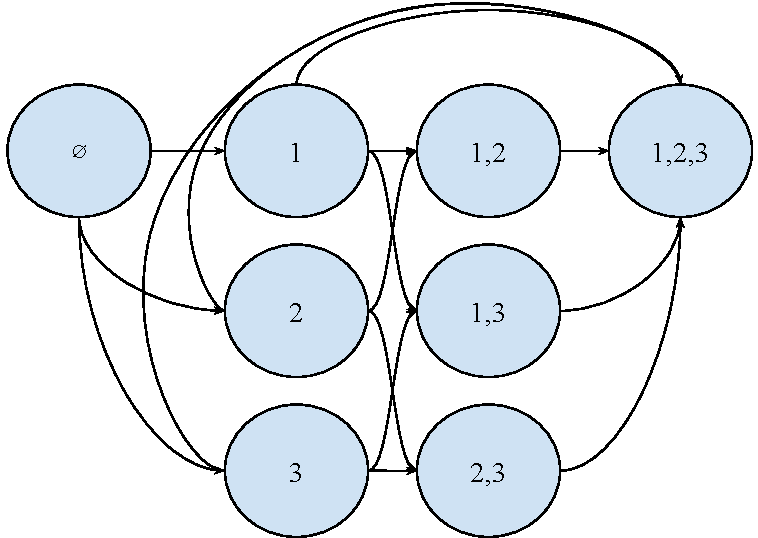
\includegraphics[width=0.75\linewidth]{MarkovStates.pdf}
\caption{Example of a Markov chain constructed for an election algorithm from information flows.}
\label{fig:markovstates}
\end{centering}
\end{figure}


The anonymous coin flipping algorithm is a useful starting point for the sorts of analysis that can be done, but presents a limited view into the potential of this type of reasoning about distributed systems. This is particularly true because of the limited practicality of the coin-flipping algorithm: each election takes approximately $log(n)$ rounds to complete, where $n$ is the total number of agents. Instead, it is more useful to do similar analysis on non-homogeneous election systems. In the following sections we present applications of this technique on an more popular election algorithm and highlight some of the potential benefits of this analysis.
With this approach we seek to have the algorithm and the interactions between agentses be memoryless so that their interactions depend only on the current state. 

\section{Application}
Analysis is presented in the context of the FREEDM DGI. The FREEDM DGI is a portion of the FREEDM project focusing on creating a distributed intelligence for controlling power electronics. As a consequence of managing the physical network of a critical infrastructure, the DGI must execute in real-time: certain actions and tasks performed by the DGI have to be completed in a specific time from.

To organize these agents, the system relies on existing clock synchronization techniques to put the system into a semi-synchronous execution environment. The DGI is divided into several modules which focus on various tasks like autonomous configuration, managing power devices and collecting data from the system. DGIs rely on synchronized clocks to begin the execution of the various tasks at the same time. This allows the message passing portions to specify deadlines to ensure that well-behaved participating agents are all working on similar tasks at the same time. For example, under the execution model as part of the autonomous configuration module, all agents begin the Leader Election Invitation Algorithm at the same time.

When reasoning about the system within the structure of the Markov Chains and MSDND security, this is a boon. An agent which is too out of sync will not be able to participate effectively and so is ignored for the purpose of this work. This effectively limits the state space of the complete naive model (as all agents are in roughly the same step of the algorithm). Furthermore, an agent can be sure that if message deliveries are timely (which is enforced by the real-time constraints) they can be certain of the lifetime of the inferred state.

This execution model has one major benefit: if, in order to participate in the algorithm, the agent must synchronize their actions (even if that synchronization is loose), the lifetime of a model is well established. In the case of a leader election algorithm, the agent that becomes the leader and constructs the model of the lifetime of the group can know for certain that another agent cannot come online and attempt to take over it's group until the next round of execution begins. A depiction of the algorithm is presented in Figures \ref{fig:statemachine} and \ref{fig:statemachine2}.

\begin{figure}[!t]
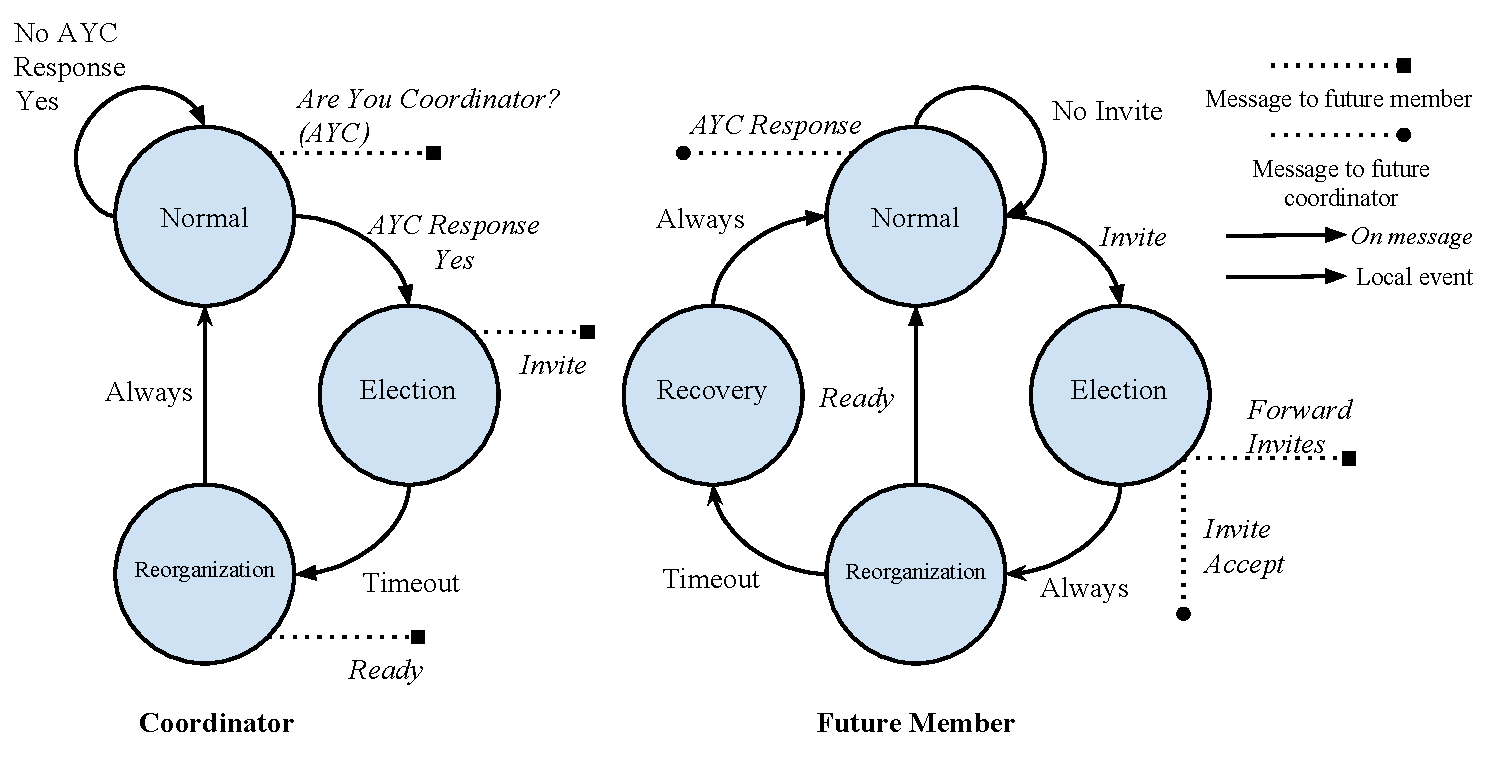
\includegraphics[width=\linewidth]{LeaderElectionStateDiagram.pdf}
\caption{State machine of a leader election. Processes start as coordinators in the ``Normal'' state and search for other coordinators to join with. Processes immediately respond to ``Are You Coordinator'' (AYC) messages they receive. The algorithm was modified by adding a ``Ready Acknowledgment'' message as the final step of completing the election. Additionally, processes only accept invites if they have received an ``AYC Response'' message from the inviting process.}
\label{fig:statemachine}
\end{figure}

\begin{figure}[!t]
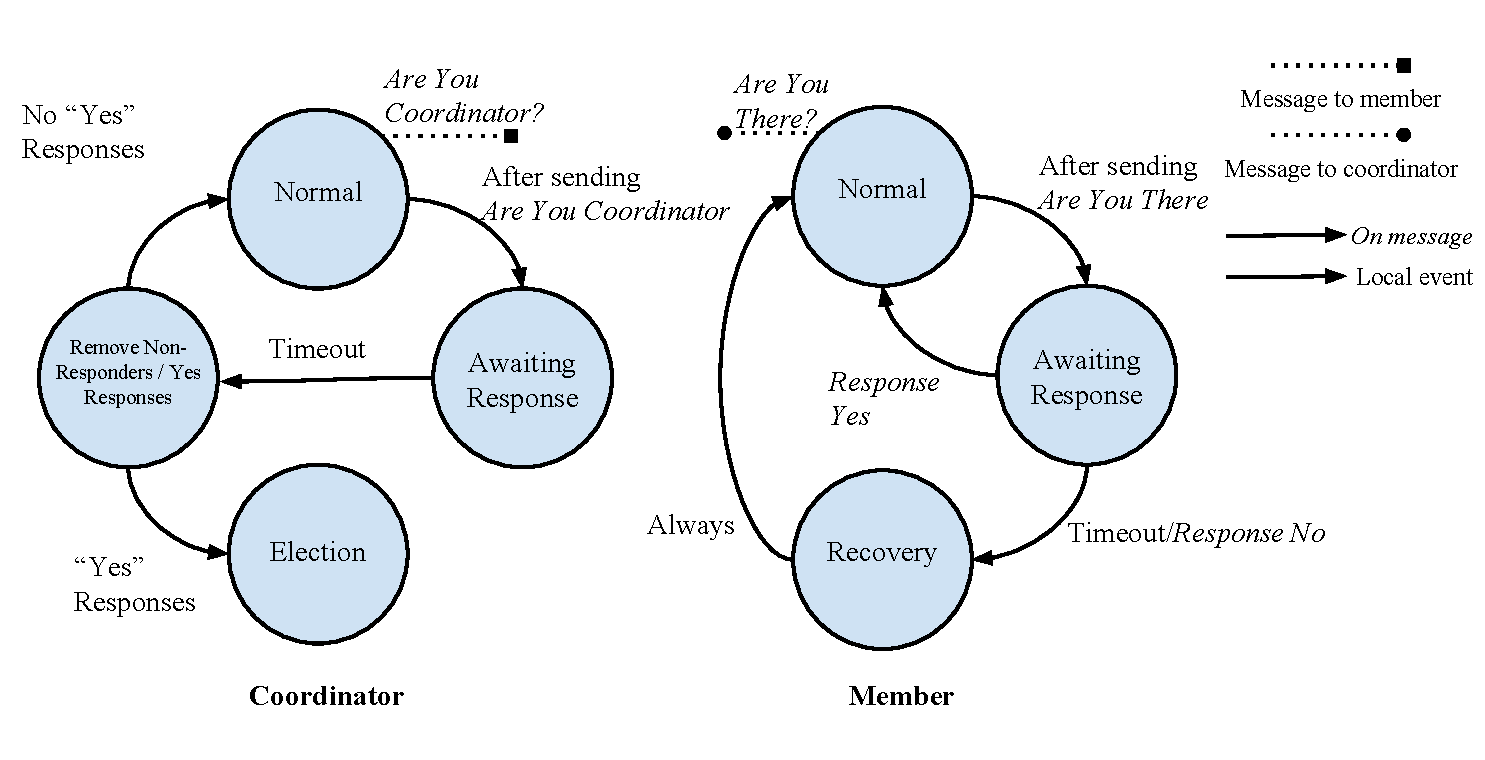
\includegraphics[width=\linewidth]{MaintainStateDiagram.pdf}
\caption{State machine of maintaining a group. The ``Are You Coordinator'' (AYC) messages are the same as those in Figure \ref{fig:statemachine}. AYC and ``Are You There'' (AYT) are periodically sent by processes, and responses to those messages are immediately sent by the receiving process. In the modified algorithm, the member does not enter the recovery state if they do not receive an AYT response before the timeout expires.}
\label{fig:statemachine2}
\end{figure}


In the following portions of the paper we present an analysis of the information leakage for the original Garcia-Molina Invitation election algorithm and present how our modified version uses the MSDND information leakage to place certainty at one agent in order to construct a Markov model. In particular, we wish to use the MSDND model to show that the changes show that the coordinator can infer if each agent in the group considers itself a part of that agent's group.

Since any coordinated actions by a group must be initialized by the coordinator, having a model of the system constructed by the coordinator is the most valuable in the context of the system. The model constructed by this approach follows the $Q$ state of the system. The $Q$ state logically underestimates the state of the system, which is more accurate with respect to determining the current state for the next step of the algorithm. For the formulas presented, the coordinator of each group constructs a model of the system based on the cardinality of the the $Q$ set based on the information flows in the algorithm.

\subsection{Group Maintenance and Leader Discovery}

The original and modified Garcia-Molina invitation election algorithms both use a common set of variables at each agent to track the state of the system.

\begin{algorithmic}[1]
\small
\State $AllNodes \gets \{ 1, 2, ..., N \}$
\State $Coordinators \gets \emptyset$
\State $UpNodes \gets { Me }$
\State $State \gets Normal$
\State $Coordinator \gets Me$
\State $Responses \gets \emptyset$
\State $Counter \gets$ A random initial identifier
\State $GroupID \gets (Me,Counter)$

\end{algorithmic}

Additionally, both versions use a recovery algorithm to abandon failed elections and groups.

\begin{algorithmic}[1]
\small
\Function{Recovery}{}
    \State $State \gets Election$
    \State Stop Work
    \State $Counter \gets Counter + 1$
    \State $GroupID \gets (Me,Counter)$
    \State $Coordinator \gets Me$
    \State $UpNodes \gets {Me}$
    \State $State \gets Reorganization$
    \State $State \gets Normal$
\EndFunction
\end{algorithmic}

\subsubsection{Original Algorithm}

\begin{algorithmic}[1]
\small
\Function{Check}{}
    \State This function is called periodically by the leader
    \If {$State = Normal$ and $Coordinator \gets Me$}
        \State $Responses \gets \emptyset$
        \State $TempSet \gets \emptyset$
        \For {$j = (AllNodes - \{Me\})$}
            \State $AreYouCoordinator(j)$
            \State $TempSet \gets TempSet \cup j$
        \EndFor
        \State Nodes which respond "Yes" to $AreYouCoordinator$ are put into the $Responses$ set. When all nodes have responded or after $Timeout(CheckTimeout)$, Nodes that do not respond are removed from UpNodes and execution continues
        \State $UpNodes \gets (TempSet-Responses) \cup {Me}$
        \If {$Responses = \emptyset$}
            \Return
        \EndIf
        \State $p \gets \max(Responses)$
        \If $Me < P$
            \State Wait time proportional to p-i
        \EndIf
        \Call{Merge}{Responses}
    \EndIf
    \State The next call to this is after Timeout(CheckTimeout)
\EndFunction

\State

\Function{RecieveAreYouCoordinator}{Sender}
    \If {$State = Normal$ and $Coordinator = Me$}
        \State Respond Yes
    \Else
        \State Respond No
    \EndIf
\EndFunction

\end{algorithmic}

The "Are Coordinator" message serves as a failure detector for crashed processes. In the models presented in this paper, crash failures are ignored as part of the modeled system.

\begin{algorithmic}[1]
\small
\Function{Timeout}{}
    \State This function is called periodically by the group members
    \If {$Coordinator = Me$}
        \Return
    \Else
        \Call{AreYouThere}{Coordinator,GroupID,Me}
        \If{Response is No or after $Timeout(TimeoutTimeout)$}
            \Call{Recovery}{}
        \EndIf
    \EndIf
    \State The next call to this is after Timeout(TimeoutTimeout)
\EndFunction

\State

\Function{RecieveAreYouThere}{Sender, Identifier}
    \If {$GroupID = Identifier$ and $Coordinator = Me$ and $Sender \in UpNodes$}
        \State Respond Yes
    \Else
        \State Respond No
    \EndIf
\EndFunction

\end{algorithmic}

The "Are You There" message serves as a check for the "Ready" message sent by the group leader at the end of the election algorithm. Are you there verifies the leader considers the sending process a part of its group.

\subsubsection{Modified Algorithm}
In the maintenance portion of the algorithm, the leader acts on the set $Q$, attempting to invite the agents not in its group into the group. Agents in $R$ but not $Q$ will be re-invited. From the messages they receive from the leader the agents in $R-Q$ will be able to infer that they are not a part of $Q$. To accomplish this, the membership state of the process can be provided to the recipient as part of the "Are You Coordinator" message or it can be inferred from the process based on the response from an AYT message.

\begin{algorithmic}[1]
\small
\Function{Check}{}
    \State This function is called at the start of a round by a leader
    \If {$State \neq Normal$ or $Coordinator \neq Me$}
        \Return
    \EndIf
    \State $Expected \gets \emptyset$
    \For {$j \in (AllPeers - \{Me\})$}
        \State $AreYouCoordinator(j)$
        \State $Expected \gets Expected \cup j$
    \EndFor
    \State Peers which respond ``Yes'' to $AreYouCoordinator$ are put into the $Coordinators$ set.
    \State Processes that respond are removed from $Expected$.
    \State When an $AreYouThere$ response is ``No'' and this process is a coordinator, the querying process is put in the $Coordinators$ set.
    \State Wait for responses, Peers that do not respond are removed from UpPeers.
    \State $UpPeers \gets (UpPeers-Expected) \cup {Me}$
    \State $UpPeers \gets (UpPeers-Coordinators) \cup {Me}$
    \If {$Responses = \emptyset$}
        \Return
    \EndIf
    \If {$Me < min(Responses)$}
        \State
        \Call{Merge}{Responses}
    \EndIf
\EndFunction

\State

\Function{ReceiveAreYouThere}{Sender, Identifier}
    \If {$GroupID = Identifier$ and $Coordinator = Me$ and $Sender \in UpPeers$}
        \State Respond Yes
    \Else
        \State Respond No
        \State $Coordinators \gets Sender$
    \EndIf
\EndFunction
\end{algorithmic}

This approach allows the memorylessness property for the imaging to be upheld. If an agent is not in $Q$ that agent will be able to determine it is not in $Q$. This allows the same number of messages to be exchanged regardless of an agent's membership in $Q$. If the probability that any given message sent to a process has a consistent probability of being delivered, the sequences of worlds that merge two coordinators has the same distribution of probable outcomes as the sequences of worlds that a process in $R$ but not $Q$ is invited to the group.


\subsection{Coordinator Priority}

Because elections can be triggered simultaneously, (and they always are in a synchronized execution model), a race condition exists in selecting the coordinator. In the original algorithm, the race condition was resolved using the agent id and a wait sequence. The agent that believed it had the lowest identification would immediately send invites, all other agents would wait some period of time before before sending theirs, in case the sender crashed. Our approach uses the maintenance and discovery phase to determine if an agent is the highest priority.

\subsubsection{Original Algorithm}

In the original algorithm, the break the race condition, each coordinator that has identified other coordinators to merge will determine if it should wait or immediately invite each process it has identified as another coordinator. This action allows the processes to avoid sending all their invites at the same time.

The original text is vague on how this condition should be determined: if the coordinators should determine their wait time based on the global list of processes that could potential become leaders or if should be determined from the set of coordinators that that agent has identified as a fellow coordinator. In either case, the selection of when to send the invites influenced heavily by timing differences between the processes leading to non-deterministic behavior in many scenarios.

\subsubsection{Modified Algorithm}

Querying an agent to see if they are a coordinator implies that the sending agent is a coordinator and implies that if that agent is not in a group with that agent and the querying agent is a coordinator, the receiving agent should expect to receive an invite from that agent, and will accept it if it is not already in a higher priority group, and it does not receive a message from a higher priority agent.

This approach of identifying priority during the group discovery phases allows the processes to determine when to send invites based on a deterministic measure rather than a probabilistic one based on execution ordering. A process can decide which invite it wishes to accept before the invites are sent out. There is a potential for live-lock in this approach if the highest priority process always crashes after other processes have determined they should accept that processes invite, but a similar scenario also exists in the original algorithm.

\subsection{Invitations}

\subsubsection{Original Algorithm}

\begin{algorithmic}[1]
\small
\Function{Merge}{Coordinators}
    \State This function invites all coordinators in Coordinators to join a group led by Me
    \State $State \gets Election$
    \State Stop work
    \State $Counter \gets Counter+1$
    \State $GroupID \gets (Me,Counter)$
    \State $Coordinator \gets Me$
    \State $TempSet \gets UpNodes - {Me}$
    \State $UpNodes \gets \emptyset$
    \For {$j \in Coordinators$}
        \Call{Invite}{j,Coordinator,GroupID}
    \EndFor
    \For {$j \in TempSet$}
        \Call{Invite}{j,Coordinator,GroupID}
    \EndFor
    \State Wait for $Timeout(InviteTimeout)$, Nodes that accept the invite are added to UpNodes
    \State $State \gets Reorganization$
    \For {$j \in UpNodes$}
        \Call{Ready}{j,Coordinator,GroupID,UpNodes}
    \EndFor
    \State $State \gets Normal$
\EndFunction

\State

\Function{RecieveInvitation}{Sender,Leader,Identifier}
    \If {$State \neq Normal$}
        \Return
    \EndIf
    \State Stop Work
    \State $Temp \gets Coordinator$
    \State $TempSet \gets UpNodes$
    \State $State \gets Election$
    \State $Coordinator \gets Leader$
    \State $GroupID \gets Identifier$
    \If {$Temp = Me$}
        \State Forward invite to old group members
        \For $j \in TempSet$
            \State $Invite(j,Coordinator,GroupID)$
        \EndFor
    \EndIf
    \State $Accept(Coordinator,GroupID)$
    \State $State \gets Reorganization$
    \If {$Timeout(ReadyTimeout)$ expires before $Ready$ is recieved}
        \State $Recovery()$
    \EndIf
\EndFunction

\Function{RecieveAccept}{Sender,Leader,Identifier}
    \If {$State \gets Election$ and $GroupID = Identifier$ and $Coordinator = Leader$}
        \State $UpNodes \gets UpNodes \cup {Sender}$
    \EndIf
\EndFunction

\State

\end{algorithmic}

\subsubsection{Modified Algorithm}

In the invitation portion of the algorithm, the sender of the invite is confident the agent has accepted the invite because the accept message arrives. The group list that the new leader prepares for the ready message is an $S$ set of the potential group members. The list is distributed to the new members. Agents that do not receive $S$ or fail to send a receipt message are not in $Q$. Algorithms that depend on the the set of agents in the group will act on $S$. There is a potential that to the leader the agents in $S$ but not $Q$ will act as though they are part of the group. Algorithmically, the the leader can then expand $Q$ to cover the information leaked by that agent acting as though it is holds a state that makes it part of $Q$.

\begin{algorithmic}[1]
\small
\Function{Merge}{Coordinators}
    \State This function invites all coordinators in Coordinators to join a group led by Me
    \State $State \gets Election$
    \State Stop work
    \State $Counter \gets Counter+1$
    \State $PendingID \gets (Me,Counter)$
    \State $Coordinator \gets Me$
    \State $Pending \gets UpPeers - {Me}$
    \For {$j \in Coordinators$}
        \Call{Invite}{j,Coordinator,PendingID}
    \EndFor
    \State Wait for responses, Peers that accept the invite are added to $Pending$.
    \State $State \gets Reorganization$
	\State $GroupID \gets PendingID$
	\State $UpPeers \gets Pending$
    \For {$j \in UpPeers$}
        \Call{Ready}{j,Coordinator,GroupID,UpPeers}
    \EndFor
    \State $Expected \gets UpPeers$
    \State Wait for responses, Peers that acknowledge are removed from $Expected$
    \State $UpPeers \gets UpPeers - Expected$
    \State $State \gets Normal$
\EndFunction

\Function{ReceiveInvitation}{Sender,Leader,Identifier}
    \If {$State \neq Normal$}
        \Return
    \EndIf
    \If {$Sender < Coordinator$}
        \Return
    \EndIf
    \State Stop Work
    \State $PendingID \gets Identifier$
    \State $State \gets Election$
    \State $Accept(Coordinator,Identifier)$
    \State $State \gets Reorganization$
    \If {$Ready$ is not received}
        \State $Recovery()$
    \EndIf
\EndFunction

\Function{ReceiveAccept}{Sender,Leader,Identifier}
    \If {$State \gets Election$ and $PendingID = Identifier$}
        \State $Pending \gets Pending \cup {Sender}$
    \EndIf
\EndFunction

\Function{ReceiveReadyAcknowledge}{Sender}
    \State $Pending \gets Pending \cup {Sender}$
\EndFunction

\end{algorithmic}

An agent can determine the likelihood that its group will form in a particular configuration if it is the highest priority agent. The determination of coordinator priority is determined during the check phase, then an agent can determine if it is the highest priority agent. If an agent determines it is the highest priority, it can then easily determine the probability that any given agent receives it's invite message and that the response to that invite message returns to that agent.

An agent can determine the likelihood that its group will form a particular configuration if it can determine the likelihood that agents with higher priority do not form a group with with the agents in that configuration.

If the determination of the coordinator priority reveals that an agent has a lower priority than 1 other agent, the probability that an agent accepts and invite from the agent is the probability the other agent does not recognize the other agent's priority (which is based on the delivery of the check messages).

Alternatively, if the determination of the coordinator priority reveals that an agent has a lower priority than n ($n > 2$) other agents, the probability that some other agent will accept that agents invite is the probability that for each of the other agents ($n-1 ... 0$) the invited agent does not recognize that agent's priority.

\subsection{Ready State}

\subsubsection{Original Algorithm}

In the original algorithm the list of processes in the group is distributed as part of the ready message. Based on analysis presented earlier in the paper, since there is no confirmation of receipt for the ready message, the leader cannot determine the actual state of the group has it only has the un-valuateable set of wffs describing the group state $S_i$.

\subsubsection{Modified Algorithm}

In the modified algorithm, the processes that receive the ready message reply with confirmation. This allows the leader of the group to determine $Q_i$, a set of processes that have definitely received the ready message. By coupling this with the other modifications to the algorithm, for the semi-synchronous execution environment used by the DGI, the states observed by the leader are memoryless.

\subsection{Expression As Markov Chain}

In the specified execution environment, each time before the coordinator runs the the check portion of the election algorithm it produces an image of the current world to use as the first state of the constructed Markov chain. Each agent in the system has the stability property. As part of the stability property any wffs whose information was transferred after the last image was taken cannot change until the process takes the newest image. For the election algorithm, this causes the leader to doubt the values in $Q$.

If a process is not in $Q$ it will have to go through the election procedure even though it may be in $R$. This ensures that the sequence of changes necessary to bring that agent into the group is identical whether regardless of the agent's membership in $R$, ensuring the memorylessness property.

% TODO: CORRECT THE NUMBERS

\begin{equation}
 \Pr_{M}(X=k; m) =
   \begin{cases}
    \binom{m}{k} p^{2k}(1-p^2)^{m-k}, & \text{if } 0 \leq k \leq m \\
    0,                                & \text{otherwise} \\
  \end{cases}
\end{equation}

\begin{equation}
	\Pr_{I}(Y=k; n) =
	\begin{cases}
		\binom{n}{k} p^{8k}(1-p^8)^{n-k}, & \text{if } 0 \leq k \leq n \\
		0,                                & \text{otherwise} \\
	\end{cases}
\end{equation}

Where $k$ is the number of agents remaining in a group selected from the $m$ agents in $Q$. For the $n$ agents not in $Q$, the $Pr_{I}(Y=k; n)$ is the probability than $k$ of those agents are in the next $Q$. By making the determination of leader priority deterministic and a property of the leader discovery phase, the probability of a particular leader successfully inviting a given process is determined by the probability that each agent with higher priority failed to invite the a given agent.

\begin{align} \Pr_{T}(Z=s'; n; s) = \sum_{i=0}^{s-1} &\Pr_{M}(X=i; s-1) \cdot
\nonumber \\ &\Pr_{I}(X=s'-i; n-s-1) \end{align}

Previous work JOURNAL demonstrates these formulae accurately describing the behavior of an implementation of this algorithm.

\section{Conclusion}

The analysis presented in the paper presents a useful framework for reasoning about creating models of distributed systems that tolerate omission failure. The models and structures presented allow algorithm designers to design algorithms whose behavior can be modeled with a Markov chain which is invaluable for designing critical infrastructure systems that behave reliably during failure conditions.

To do this, applied existing information flow analysis techniques and applied them to a common distributed systems problem (the two-armies problem) and show the information flow analysis was consistent with similar analyses of the problem. We then extended the analysis to show how agents in a distributed system could use that analysis to determine what knowledge each process had. As part of this we described belief sets created by distributing information to several other agents in the system.

Additionally, we defined how information being transferred between agents and the actions they take based on that information could be constrained to hold to the memorylessness property common to Markov chains. Using this concept we demonstrated how a common leader election algorithm could be modified to use this memorylessness property, allowing it to be modeled online during changing conditions.

This work is particularly valuable for the analysis of critical infrastructure systems, where knowledge of their behavior during fault conditions is particularly important. By allowing the ability for algorithms to determine what issues are likely to arise while they are operating, actions can be taken to protect the infrastructure from failure. There are a wide range of possible applications, including actions either undertaken by human operators on site, or autonomous actions taken by the algorithms to harden themselves against failure.

